\documentclass[10pt]{article}

\usepackage{graphicx}
\usepackage{amsmath}
\usepackage[ansinew]{inputenc}
\usepackage[spanish]{babel}
\usepackage{babelbib}
\usepackage[T1]{fontenc}
\usepackage[vmargin=4cm,hmargin=4cm,letterpaper]{geometry}
\usepackage{color}
\usepackage{framed}
\usepackage{hyperref}

\usepackage{listings}
\definecolor{red}{RGB}{219,0,0}
\definecolor{pink}{RGB}{255,100,100}
\definecolor{gray}{RGB}{100,100,100}
\lstset{
		basicstyle=\ttfamily,
		frame=single,
		keywordstyle=\color{red},
		commentstyle=\color{gray},
		stringstyle=\color{pink},
		tabsize=3,
		language=verilog,
		backgroundcolor=\color{white}}

\usepackage{fancyhdr} 
\pagestyle{fancy}
\usepackage{lastpage}
\lhead{Laboratorio 2}
\chead{}
\rhead{Anteproyecto}
\lfoot{}
\cfoot{}
\rfoot{\footnotesize Page \thepage\ of \pageref{LastPage}}

\renewcommand{\headrulewidth}{0.4pt} 
\renewcommand{\footrulewidth}{0.4pt} 

\graphicspath{{../media/}}	%%multimedia path
\setlength{\parindent}{0pt}
%%*************************************************************************
\begin{document}

\begin{huge}
\begin{center}
\textbf{Laboratorio 2: Circuitos Combinatorios}
\end{center}
\end{huge}

\begin{Large}
\begin{center}
Jose Ap� (B10407), Francisco Molina (B12345), \\Marco Montero (A94000), Dennis Vargas (B16831)
\end{center}
\end{Large}


\section*{Ejercicio 1}
Se agreg� e implemento la operaci�n SMUL al experimento 1 de distintas formas, multiplicando los valores de src1 y src2 y guardando el resultado en dst. Se compar� las frecuencias, adem�s del n�mero de LUTs, Slices y Flip-Flops. Para este primer ejercicio se prob� utilizando el operador *, tanto para multiplicaci�n sin signo como para multiplicaci�n con signo. \\[0.3 cm]
Para la multiplicaci�n sin signo se obtuvieron los resultados de las figuras \ref{freq1} y \ref{mux1}. 
\begin{figure}[hbtp]
\centering
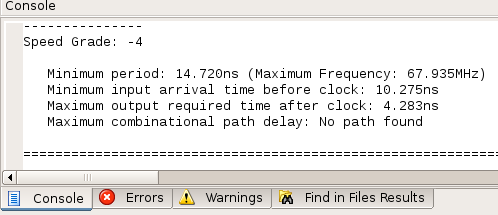
\includegraphics[width=12 cm]{../media/mul_max_freq.png}
\caption{Frecuencia m�xima del operador * sin signo}
\label{freq1}
\end{figure}

\begin{figure}[hbtp]
\centering
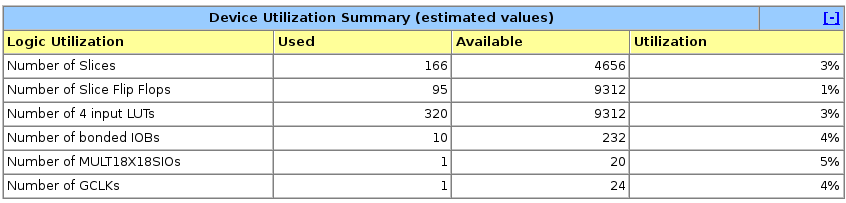
\includegraphics[width=12 cm]{../media/mul_table.png}
\caption{ LUTs, Slices y Flip-Flops del operador * sin signo}
\label{mux1}
\end{figure}
\newpage

Para la multiplicaci�n con signo primero se prob� que efectivamente se estaba realizando la operaci�n correctamente con la figura  \ref{signed} y luego se obtuvieron los resultados de las figuras \ref{freq1a} y \ref{mux1a}. 

\begin{figure}[hbtp]
\centering
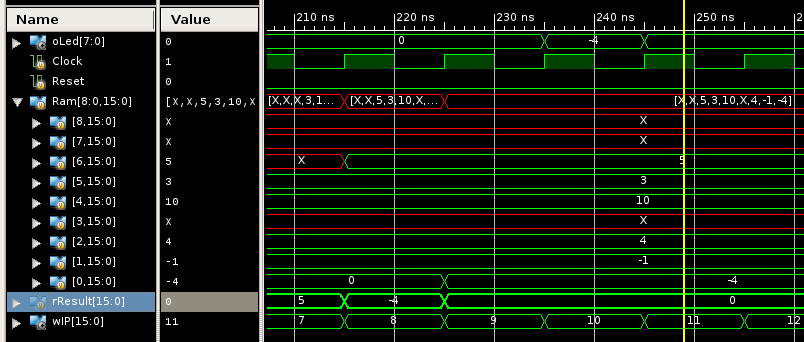
\includegraphics[width=12 cm]{../media/sim_mul_signed.png}
\caption{Prueba multiplicaci�n con signo}
\label{signed}
\end{figure}

\begin{figure}[hbtp]
\centering
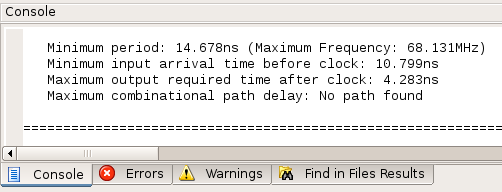
\includegraphics[width=12 cm]{../media/wo_mul_max_freq.png}
\caption{Frecuencia m�xima del operador * sin signo}
\label{freq1a}
\end{figure}

\begin{figure}[hbtp]
\centering
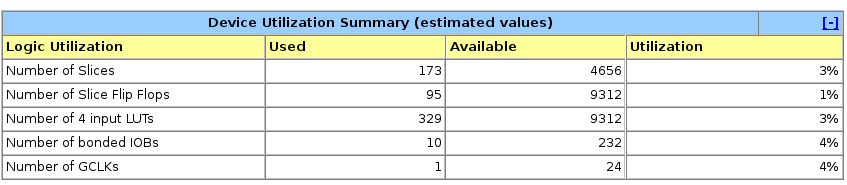
\includegraphics[width=12 cm]{../media/wo_mul_table.png}
\caption{ LUTs, Slices y Flip-Flops del operador * sin signo}
\label{mux1a}
\end{figure}
\newpage

\section*{Ejercicio 2}
Los bloques de multiplicaci�n del FPGA son adem�s capaces de llevar acabo multiplicaci�nes con signo (con n�meros representados en complemento a 2). Para esto es
necesario que la herramienta de s�ntesis entienda que las lineas de entrada a los puertos del multiplicador tienen signo. \\Esto se hace de la siguiente manera:
\begin{lstlisting}
wire [9:0] wA, wB;
wire [31:0] R = wA * wB; //multiplicaci�n sin signo
wire signed [15:0] wA, wB;
wire signed [31:0] wR = wA * wB; // multiplicaci�n con signo
\end{lstlisting}
Note en la figura siguiente como el simulador reconoce la multiplicaci�n con signo:
\begin{figure}[hbtp]
\centering
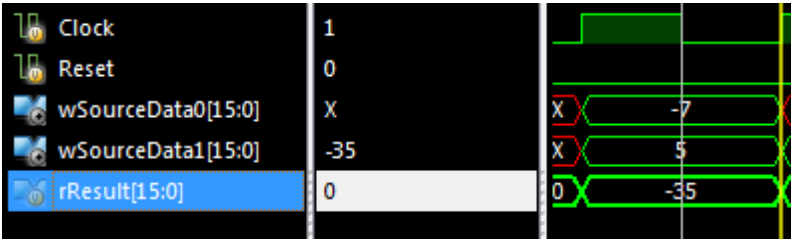
\includegraphics[width=12 cm]{../media/r1.png}
\caption{}
\label{p1}
\end{figure}

\section*{Ejercicio 3}
Usando generate se pudo hacer una m�ltiplicaci�n de 16 bits. Se utiliz� el siguiente c�digo para este ejercicio:

\begin{lstlisting}
parameter n=8;//numero de bits nxn a multiplicar
wire [n:0] wCarryTable[n-2:0];  
wire [n:0] wYout[n-2:0];
wire [15:0] wA,wB;
wire [(2*n-1):0] Resultado;

assign Resultado[0]=wSourceData0[0]&wSourceData1[0];
assign wA=wSourceData0;
assign wB=wSourceData1;

genvar CurrentCol,CurrentRow,i;
generate
	for(CurrentRow=0;CurrentRow<(n-1);CurrentRow=CurrentRow+1)
		begin: Loop1
		assign wCarryTable[CurrentRow][0]=0;
		for(CurrentCol=0;CurrentCol<n;CurrentCol=CurrentCol+1)
			begin:Loop2
			if(CurrentRow==0)//Para la primera fila
				begin:if1
				assign  wA[n]=0;//La entrada cero del sumador la ultima columna 
				ADDER myadd(
				.iA(wA[CurrentCol+1]&wB[CurrentRow]),
				.iB(wA[CurrentCol]&wB[CurrentRow+1]),
				.iCarry(wCarryTable[CurrentRow][CurrentCol]),
				.oCarry(wCarryTable[CurrentRow][CurrentCol+1]),
				.oY(wYout[CurrentRow][CurrentCol])
				);
				end
			else//Las otras filas
				begin:if1
				assign wYout[CurrentRow-1][n]=wCarryTable[CurrentRow-1][n];
				ADDER myadd1(
				.iA(wA[CurrentCol]&wB[CurrentRow+1]),
				.iB(wYout[CurrentRow-1][CurrentCol+1]),
				.iCarry(wCarryTable[CurrentRow][CurrentCol]),
				.oCarry(wCarryTable[CurrentRow][CurrentCol+1]),
				.oY(wYout[CurrentRow][CurrentCol])
				);
				end
			end//Finaliza lazo interno.

//Para llenar los bit de "Resultado" independientemente del numero de bits "nxn" a multiplicar.	
		assign Resultado[CurrentRow+1]=wYout[CurrentRow][0];
		if(CurrentRow==(n-2))
			begin:if3
			for(i=1;i<n;i=i+1)
				begin:loop3
				assign Resultado[(CurrentRow+1+i)]=wYout[CurrentRow][i];
				end
			end
		
	end//Finaliza lazo externo
assign Resultado[(2*n-1)]=wCarryTable[n-2][n];//Ultimo bit de acarreo	
endgenerate

\end{lstlisting}

Y luego se prob� la multiplicaci�n de dos n�meros 10 * 18  y se observ� el resultado en los leds de la spartan 3E.
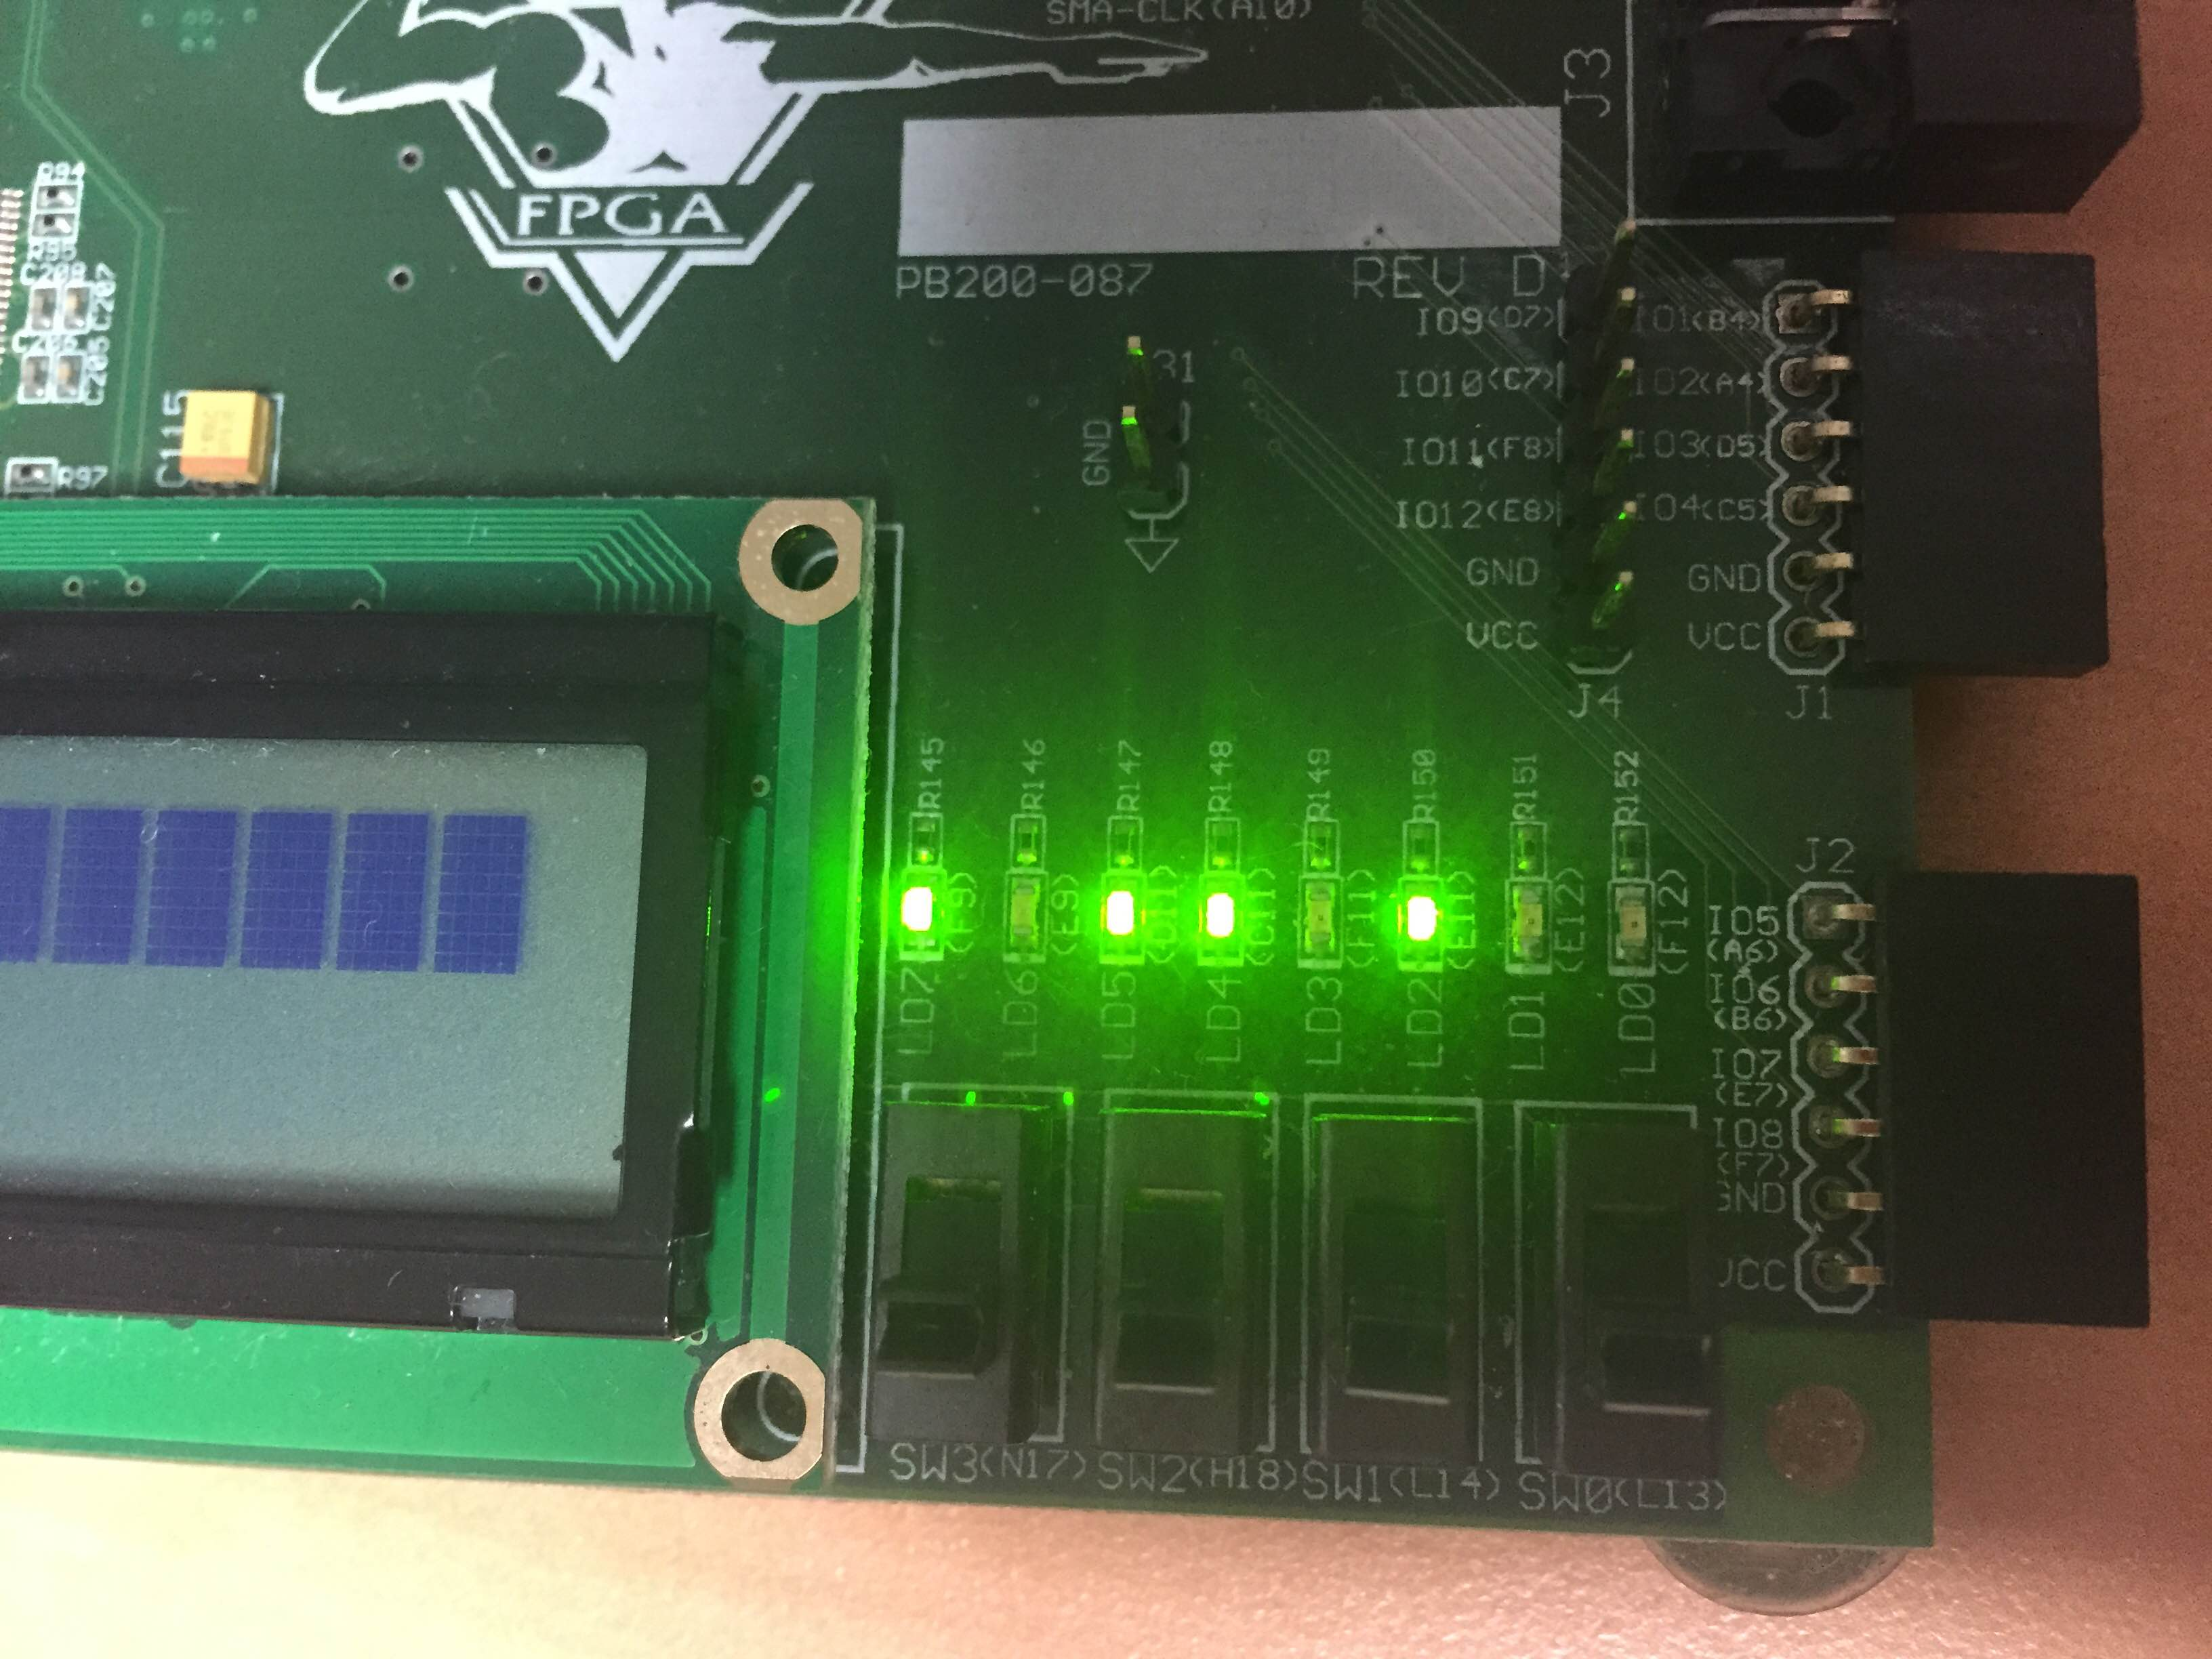
\includegraphics[width=14cm]{../media/180GMUL.JPG}

\pagebreak 
\section*{Ejercicio 4}
Luego de una serie de pruebas se determin� cual es la cantidad de espacios que se debe desplazar cada resultado parcial para multiplicar n�meros con m�s de 2 bits. En la figura \ref{p2} se muestra la estrucutura implementada para multiplicar n�meros de 8 bits y siguiendo la misma l�gica se puede obtener f�cilmente una funci�n para multiplicar 16 bits o inclusive m�s.
\begin{figure}[hbtp]
\centering
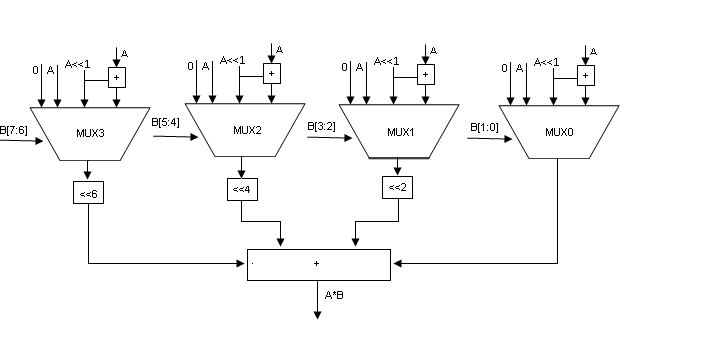
\includegraphics[width=14 cm]{../media/Muxed.png}
\caption{Multiplicador 8 bits con LUT}
\label{p2}
\end{figure}

\section*{Ejercicio 5}
Para implementar un multiplexor que codifique una LUT de 4 bits, se debe cumplir la tabla de verdad del cuadro \ref{t1}. Si se observa con detenimiento en la tabla, se logra identificar un patr�n en el resultado de las multiplicaciones. 
Una ventaja de utilizar este multiplexor es que se necesitar�n menos m�dulos para multiplicar n�meros de mayor cantidad de bits. Por ejemplo, con el mux implementado en el ejercicio anterior para multiplicar n�meros de 8 bits se necesitr�an 4 multiplexores, mientras que utlizando este nuevo multiplexor, solamente es necesario utilizar 2.
Una posible desventaja es que a la hora de multiplicar n�meros mayores a 4 bits, se puede tornar un poco engorroso identificar cuantos posiciones a la izquierda se debe desplazar cada subresultado de 4 bits.

\begin{table}[h!]
\centering 
\caption{Tabla de verdad de Mux para LTU de 4 bits}
\begin{tabular}{cl}
\hline
 B(4 bits) &        AxB \\
\hline
      0000 &          0 \\

      0001 &          A \\

      0010 &       A$<<$1 \\

      0011 &   (A$<<$1)+A \\

      0100 &       A$<<$2 \\

      0101 &   (A$<<$2)+A \\

      0110 & (A$<<$2)+(A$<<$1) \\

      0111 & (A$<<$2)+(A$<<$1)+A \\

      1000 &       A$<<$3 \\

      1001 &   (A$<<$3)+A \\

      1010 & (A$<<$3)+(A$<<$1) \\

      1011 & (A$<<$3)+(A$<<$1)+A \\

      1100 & (A$<<$3)+(A$<<$2) \\

      1101 & (A$<<$3)+(A$<<$2)+A \\

      1110 & (A$<<$3)+(A$<<$2)+(A$<<$1) \\

      1111 & (A$<<$3)+(A$<<$2)+(A$<<$1)+A \\

\end{tabular}  
\label{t1}
\end{table}


\end{document}
%%*************************************************************************
